\chapter{Evaluation and Results}
\label{ch:evaluation-and-results}

% \section{Introduction}
\section{Evaluation Setup}
\label{sec:evaluation-setup}
% How everything was set up (kubernetes, ml,...)

  In this section the evaluation setup will be described in detail. 
  This involves what tools and technologies were used and how they were combined in order to evaluate our test cases. Additionally, the \nameref{sec:forecasting-metrics-evaluation-setup} that are used are briefly described since they are crucial for the forecast prediction performance comparisons.
  
  \subsection{Docker}
  \label{sec:docker-evaluation-setup}

    Docker is an open-source platform for automating the deployment of applications inside containers. A container is a standalone executable package that includes everything needed to run a piece of software, including the code, runtime, libraries, environment variables, and system tools.
    Abstracting applications as containers provide a consistent and reproducible environment, which makes it easier to move applications between development, testing and production environments.
    Containers are often used to package an entire application with all it's dependencies into a single container image that can easily be moved and run on any device with a Docker runtime.
    The docker toolbox provides tools for building, shipping and running containers, including a runtime environment for containers called Docker Engine, Docker Hub (a repository for storing and sharing images) and the Docker CLI to be able to interact with Docker via a command-line interface.



  \subsection{Kubernetes}
  \label{sec:kubernetes-evaluation-setup}
    Kubernetes is an open-source platform for automating deployment, scaling, and management of containerized applications. It was originally developed by Google and is now maintained by the Cloud Native Computing Foundation (CNCF).
    Kubernetes provides a way to manage and organize containers (such as \nameref{sec:docker-evaluation-setup} containers) at scale, making it easier to deploy, update, and maintain applications. It does this by abstracting the underlying infrastructure and providing a unified API for managing containers.
    Kubernetes helps to automate many of the manual tasks involved in deploying and managing containers, such as scaling up or down the number of replicas of an application, rolling out updates, and managing network and storage resources. It also provides features for scaling and self-healing, allowing your applications to be more robust and resilient.
    Kubernetes has become a popular platform for deploying cloud-native applications and is widely used by organizations of all sizes across various industries.

  \subsection{NetData}
  \label{sec:netdata-evaluation-setup}

    Netdata is an open source tool that collects real-time metrics, including CPU usage, disk activity, bandwidth usage and further more.
    The reason we chose Netdata for monitoring is that it is a lightweight tool mostly written in C, Python and Javascript and it requires minimal resources, which is necessary when monitoring edge devices.
    One of its major features is that it runs without interrupting any of the applications running on the same device. This is achieved by only using idle CPU cycles while running.
    Netdata provides an in-browser dashboard to analyse each metric in real time with help of visual representation. As an example, a screenshot was taken of a cloud resource in our system as can be seen in \ref{fig:netdata-dashboard}.
    \begin{figure}[h!]
        \centering
        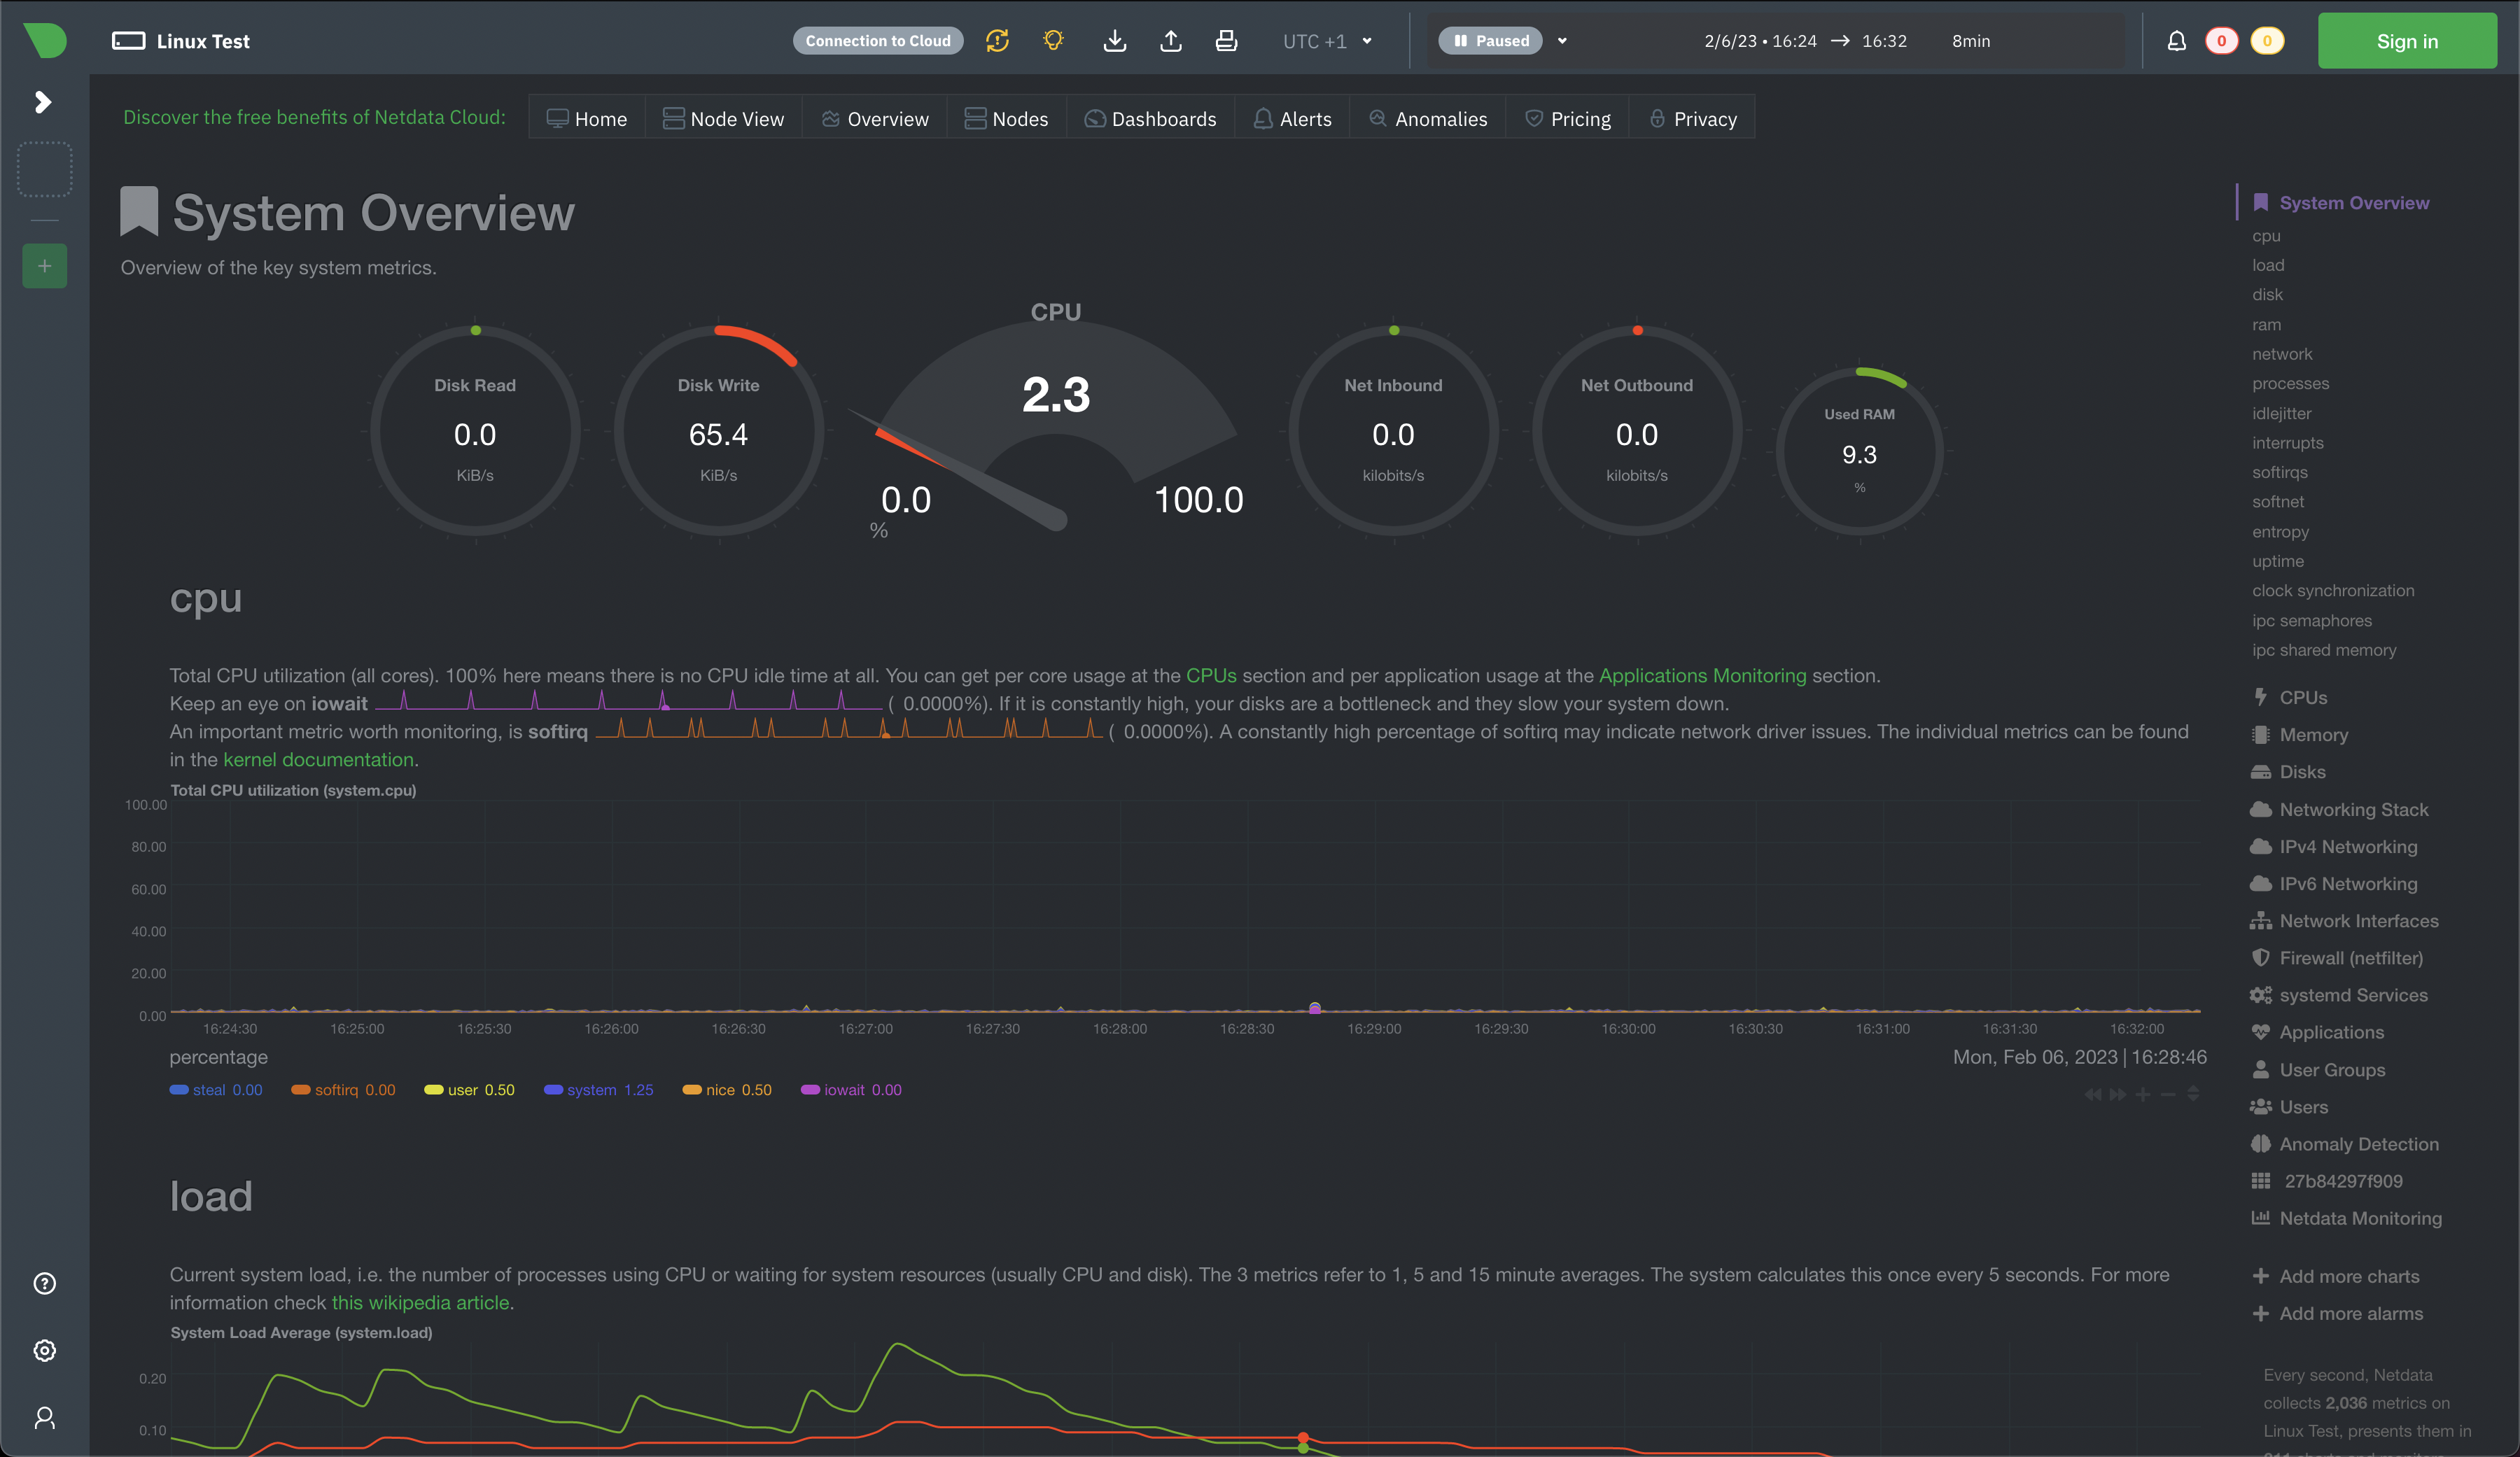
\includegraphics[width=0.95\textwidth]{figures/netdata.png}
        \caption{Netdata Dashboard Example}
        \label{fig:netdata-dashboard}
    \end{figure}
    Netdata has a vast amount of support for other tools in order to gather data. 
    One of the supported tools is \nameref{sec:prometheus-evaluation-setup}, which is used to scrape the monitored data from all resources that have Netdata installed.

  \subsection{Prometheus}
  \label{sec:prometheus-evaluation-setup}
  
    Prometheus\footnote{https://prometheus.io/} is an open source application used for monitoring and alerting of events and is designed to run across various platforms in a scalable and easily deployable manner.
    Same as Netdata it records in real-time, and stores the gathered metrics in a time series database by using a \emph{HTTP pull model}. It also allows real-time alerting via a rule defining configuration and also has a flexible query language called \emph{PromQL}, that enables the retrieval and processing the gathered data. Prometheus has great integration with other tools such as Netdata.
    In the project it is used inside a monitoring master node that is continuously scraping all resources that have Netdata installed for monitoring data. In case a predefined rule is broken at a monitored resource, such as CPU over-allocation, Prometheus triggers an event that notifies ADA-PIPE in order to be able to take measurements.

  \subsection{PyTorch}
  \label{sec:pytorch-evaluation-setup}
  \footnote{https://pytorch.org/}

  \subsection{LSTM Model Setup}
  \subsection{Forecasting Metrics}
  \label{sec:forecasting-metrics-evaluation-setup}

    Forecasting metrics are measures used to evaluate the accuracy of forecasting models. These metrics are used to compare different models, assess the quality of the forecasts, and identify areas for improvement.

    % Maybe add those metrics? 

    % Mean Absolute Error (MAE): measures the average magnitude of the error between the predicted values and the actual values.

    % Theil's U-Statistic: measures the accuracy of a forecast relative to the accuracy of a naive forecast.

    % Mean Absolute Scaled Error (MASE): measures the accuracy of a forecast relative to the accuracy of a naïve forecast.

    The choice of forecasting metric will depend on the specific goals and requirements of the forecasting task. Some metrics may be more appropriate for certain types of data or models, while others may be better suited for comparing different models.
    Overall, the use of appropriate forecasting metrics is critical for evaluating the accuracy of forecasting models and for identifying areas for improvement.

    \paragraph{MAPE}
    \label{par:mape-metrics-evaluation}
      Mean Absolute Percentage Error (MAPE) is a commonly used metric for evaluating the accuracy of forecasting models. It measures the average percentage difference between the predicted values and the actual values.
      The formula for MAPE is:

      $$MAPE = \frac{1}{n} \times \sum \left|\frac{Actual - Predicted}{Actual}\right| \times 100$$
      where $n$ denotes the number of data points and $Actual$ and $Predicted$ are the actual and predicted values, respectively.
      MAPE provides a percentage error, which makes it easy to interpret and compare the accuracy of forecasting models. 
      
      However, there are some limitations to using MAPE, such as the fact that it can become undefined when the actual value is zero (in our case if there is no resource utilisation at some time step $i$), and it can be sensitive to outliers.
      Despite these limitations, MAPE is a widely used metric for evaluating forecasting models, especially if it is important to understand the relative magnitude of the errors in the predictions. 
      Overall, MAPE provides a useful way to measure the accuracy of forecasting models and can help to identify areas for improvement in the model or the data.


    \paragraph{sMAPE}
    \label{par:smape-metrics-evaluation}
    
      Symmetric Mean Absolute Percentage Error (SMAPE) is a metric used for evaluating the accuracy of forecasting models. It measures the average percentage difference between the predicted values and the actual values, and is symmetrical in that it treats positive and negative errors equally.
      In our evaluation of the prediction performance this is especially useful since both over-, and under-utilisation are present in all prediction variants.
      The formula for SMAPE is:

      $$sMAPE = \frac{1}{n} \times \sum \left|\frac{Actual - Predicted}{\left(Actual + Predicted\right) \div 2}\right| \times 100$$
      where $n$ denotes the number of data points and $Actual$ and $Predicted$ are the actual and predicted values, respectively.
      sMAPE provides a percentage error similar to \nameref{par:mape-metrics-evaluation}, which makes it easy to interpret and compare the accuracy of forecasting models. Unlike MAPE, sMAPE is symmetrical, since it doesn't become undefined when the actual value is zero, and another difference is that it is less sensitive to outliers.
      Overall, sMAPE is a useful metric for evaluating the accuracy of forecasting models and can provide valuable information for understanding the relative magnitude of the errors in the predictions.

    \paragraph{RMSE}
    \label{par:rmse-metrics-evaluation}

      Root Mean Squared Error (RMSE) is a metric used for evaluating the accuracy of forecasting models. It measures the average magnitude of the error between the predicted values and the actual values, and provides a useful way to compare the magnitude of the errors in different models.
      The formula for RMSE is:
      $$RMSE = \sqrt{\frac{\sum_{i = 1}^{N}\left(Predicted_i - Actual_i\right)^2}{N}}$$
      where $n$ denotes the number of data points and $Actual$ and $Predicted$ are the actual and predicted values, respectively.
      RMSE provides a measure of the magnitude of the errors in the predictions, with lower values indicating a more accurate model. 
      RMSE is particularly useful when the goal is to minimize the magnitude of the errors in the predictions.
      One important thing to note about RMSE is that it is sensitive to the scale of the data. This means that it is more appropriate to use RMSE when the scale of the actual and predicted values is similar.
      Because of the scale sensitivity of RMSE, the number of actual and predicted values is equivalent for all our evaluation scenarios in order to be able to use RMSE for a comparison between different approaches.
      Overall, RMSE is a widely used and useful metric for evaluating the accuracy of forecasting models and can provide valuable information for understanding the magnitude of the errors in the predictions.

% \paragraph{Theil's U-Statistic}

% Theil's U-Statistic is a measure of the accuracy of a forecasting model relative to a naïve forecast. The naïve forecast is a simple forecast that uses the average or last observed value as the prediction for all future time points. Theil's U-Statistic is used to compare the accuracy of a forecast with the accuracy of the naïve forecast.

% The formula for Theil's U-Statistic is:

% U = (RMSE of the forecast) / (RMSE of the naïve forecast)

% where RMSE stands for Root Mean Squared Error.

% Theil's U-Statistic is a unitless measure, with values ranging from 0 to infinity. A value of 0 indicates that the forecast is no better than the naïve forecast, while a value greater than 1 indicates that the forecast is more accurate than the naïve forecast.

% Theil's U-Statistic is particularly useful when the goal is to compare the accuracy of a forecast with the accuracy of a simple, baseline forecast. It provides a useful way to evaluate the improvement in accuracy achieved by using a more sophisticated forecasting model.

% Overall, Theil's U-Statistic is a valuable tool for evaluating the accuracy of forecasting models, and for comparing the accuracy of different models relative to a simple, baseline forecast.
    \paragraph{Resource Wastage}
      Calculated by subtracting the surface area of allocated - predicted.

  \subsection{Weights \& Biases}
    
    Weights \& Biases (W\&B)\footnote{https://wandb.ai} is a software company that provides an AI platform for machine learning and deep learning. Their platform provides tools for tracking experiments, visualizing models, and collaborating with team members.
    The platform provides a centralized repository for all of the information related to a machine learning project, including code, data, models, and results.
    W\&B offers a range of features to help users better understand their models, including interactive visualizations of model architecture, weight distributions, and training metrics. The platform also provides a suite of tools for tracking experiments, which makes it easy to compare different models and understand the impact of changes to the code or data.

    % The W\&B platform is designed to make it easier for data scientists, machine learning engineers, and researchers to manage the complexity of developing and deploying machine learning models. 


    % Overall, W\&B provides a comprehensive solution for machine learning and deep learning development, and can be a valuable tool for organizations looking to streamline their machine learning operations and improve their ability to develop high-quality models.
  
\section{Evaluation Scenarios}
\label{sec:evaluation-scenarios}

% the different evaluations I did like task type or batch size

  \subsection{Simple LSTM Model}

  \subsection{Adding Task Knowledge}

  \subsection{Adding Instance Knowledge}

  \subsection{Training with Custom Loss Function}

  \subsection{Inference Time}
  \subsection{Prediction Performance depending on Batch Size}

    % Different batch sizes
    % Different models?

    
\section{Monitoring}


\section{Data Analysis}
\section{Adaptation}
